\thispagestyle{plain}

\chapter{Exploratory Data Analysis (EDA)}
\label{cp:eda}


\section{Dataset imbalance}

Observation: The visualization clearly shows that our target variable, income, is significantly imbalanced.\\

\noindent The majority class, $\le$50K, accounts for approximately 76.1\% of the dataset.\\
The minority class, $>$50K, makes up only 23.9\%.\\

Implication: This imbalance is a critical finding and has two major consequences for our project:
\begin{itemize}
    \item Evaluation Metric: Standard accuracy will be a misleading metric. A naive model that always predicts the majority class ($\le$50K) would achieve $\approx$76\% accuracy but would be completely useless. We must therefore use more robust metrics to avoid these misinformations.

    \item Modeling Strategy: We may need to employ special techniques to help our model learn from the under-represented minority class. This could involve using class weights or applying a resampling technique like SMOTE (Synthetic Minority Over-sampling Technique) during the modeling phase.
\end{itemize}

\subsection{Metric we choose}

While the F1-Score is a popular metric for imbalanced datasets, we have chosen the \textbf{Matthews Correlation Coefficient (MCC)} as our primary metric for model selection. This decision is based on a critical mathematical distinction we found on
The Matthews correlation coefficient
(MCC) is more reliable than balanced
accuracy, bookmaker informedness, and
markedness in two-class confusion matrix
evaluation%\footcite{Chicco2021} :
\begin{enumerate}
    \item \textbf{Symmetry vs. Asymmetry:} 
    The F1-Score represents the harmonic mean of Precision and Recall. It focuses almost exclusively on the positive class (the minority class). It ignores the count of True Negatives (TN). 
    
    In our context, correctly identifying people earning $\le$50K (True Negatives) is also important to avoid false positives. The MCC, on the other hand, is symmetric. It treats both classes (high and low income) with equal importance.
    
    \item \textbf{Robustness to Class Swapping:} 
    If we were to swap the positive and negative classes (i.e., try to predict who earns $\le$50K instead of $>$50K), the F1-Score would change drastically. The MCC would remain exactly the same. This invariance makes MCC a more reliable indicator of the model's overall predictive power, regardless of which class is defined as "positive."
    
    \item \textbf{Mathematical Completeness:} 
    MCC is effectively a correlation coefficient between the observed and predicted binary classifications. It utilizes all four quadrants of the confusion matrix ($TP, TN, FP, FN$), whereas F1-Score utilizes only three ($TP, FP, FN$).
\end{enumerate}

\begin{table}[h]
    \centering
    \begin{tabular}{ll}
        \toprule
        \textbf{MCC Value} & \textbf{Interpretation} \\
        \midrule
        $< 0.20$      & Very Weak / Negligible \\
        $0.20 - 0.39$ & Weak \\
        $0.40 - 0.59$ & Moderate \\
        $0.60 - 0.79$ & Strong \\
        $\ge 0.80$    & Very Strong \\
        \bottomrule
    \end{tabular}
    \label{tab:mcc_interpretation}
    \caption{Interpretation of the Matthews Correlation Coefficient (MCC).}
\end{table}


\section{Dealing with missing values}

We have identified that the NaN values in workclass are not random, they have a distinct income distribution (90.5\% $\le$50K).
We must now decide on a handling strategy. A common method is to impute (replace) NaN values with the column's mode. We will test if this is a valid approach.\\

Hypothesis: If the income distribution of the mode category is similar to our NaN group, imputation is a good strategy.\\

Alternative: If the distribution is different, imputing with the mode would be incorrect and introduce bias. We would then need to consider another strategy, such as removing the rows or creating a new 'Unknown' category.\\

\noindent Our analysis revealed a critical insight: the missing values are not random.\\

\noindent We found: 
\begin{itemize}
    \item The NaN group for workclass has a unique income distribution (90.5\% $\le$50K), which is vastly different from the dataset's average (76.1\% $\le$50K).

    \item Imputing with the mode ('Private', at 78.2\% $\le$50K) would be incorrect. It would wrongly assign this distinct group to a category with a much higher earning rate, thereby damaging our model.
\end{itemize}

\noindent Decision for Feature Engineering:

\begin{itemize}
    \item Instead of deleting these rows (and losing $\approx$5.7\% of our data) or imputing incorrectly, our best strategy is to treat this "missingness" as an informative feature.

    \item During the Feature Engineering phase, we will create a new, distinct category called 'Unknown' (or similar) to replace these NaN values. This will allow our model to learn from this group, as their "unknown" status appears to be a strong predictor of lower income.
\end{itemize}

\section{Analysis of age distribution}

\begin{figure}[H]
    \centering
    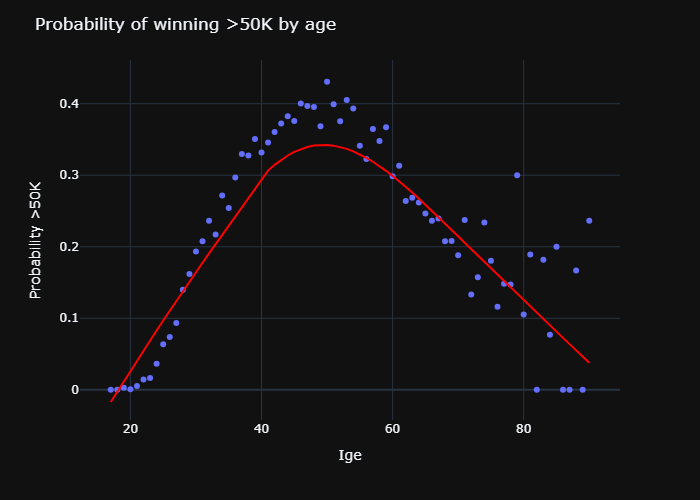
\includegraphics[width=0.8\textwidth]{Images/age.png}
    \caption{Relation between age and income}
    \label{fig:distribution_age}
\end{figure}

\vspace{2\baselineskip}

\textbf{Observations:}
Visual analysis highlights two critical issues for raw numerical modeling:
\begin{enumerate}
    \item \textbf{Outliers in the Upper Tail:} The distribution is heavily right-skewed, with sparse data points (outliers) located at the end of the graph ($>70$ years), which can negatively impact model stability.
    \item \textbf{Bell-Shaped Relationship:} Crucially, the correlation with income is \textbf{non-monotonic}. The probability of earning $>50K$ follows a "bell curve": it is low for young entrants, peaks during mid-career, and drops significantly after retirement.
\end{enumerate}

\textbf{Feature Engineering Strategy:}
A standard linear model cannot capture this "rise-and-fall" pattern using a single coefficient, it would attempt to fit a straight line through this curve, leading to significant underfitting.

Therefore, \textbf{Binning (Discretization)} is the optimal solution. By segmenting age into categorical buckets (e.g., \textit{Young, Active, Senior}), we solve both problems simultaneously: we group the sparse outliers into a robust "Senior" category and allow the model to learn a specific weight for the high-income "Active" peak.

\section{Analysis of native country}

\begin{figure}[H]
    \centering
    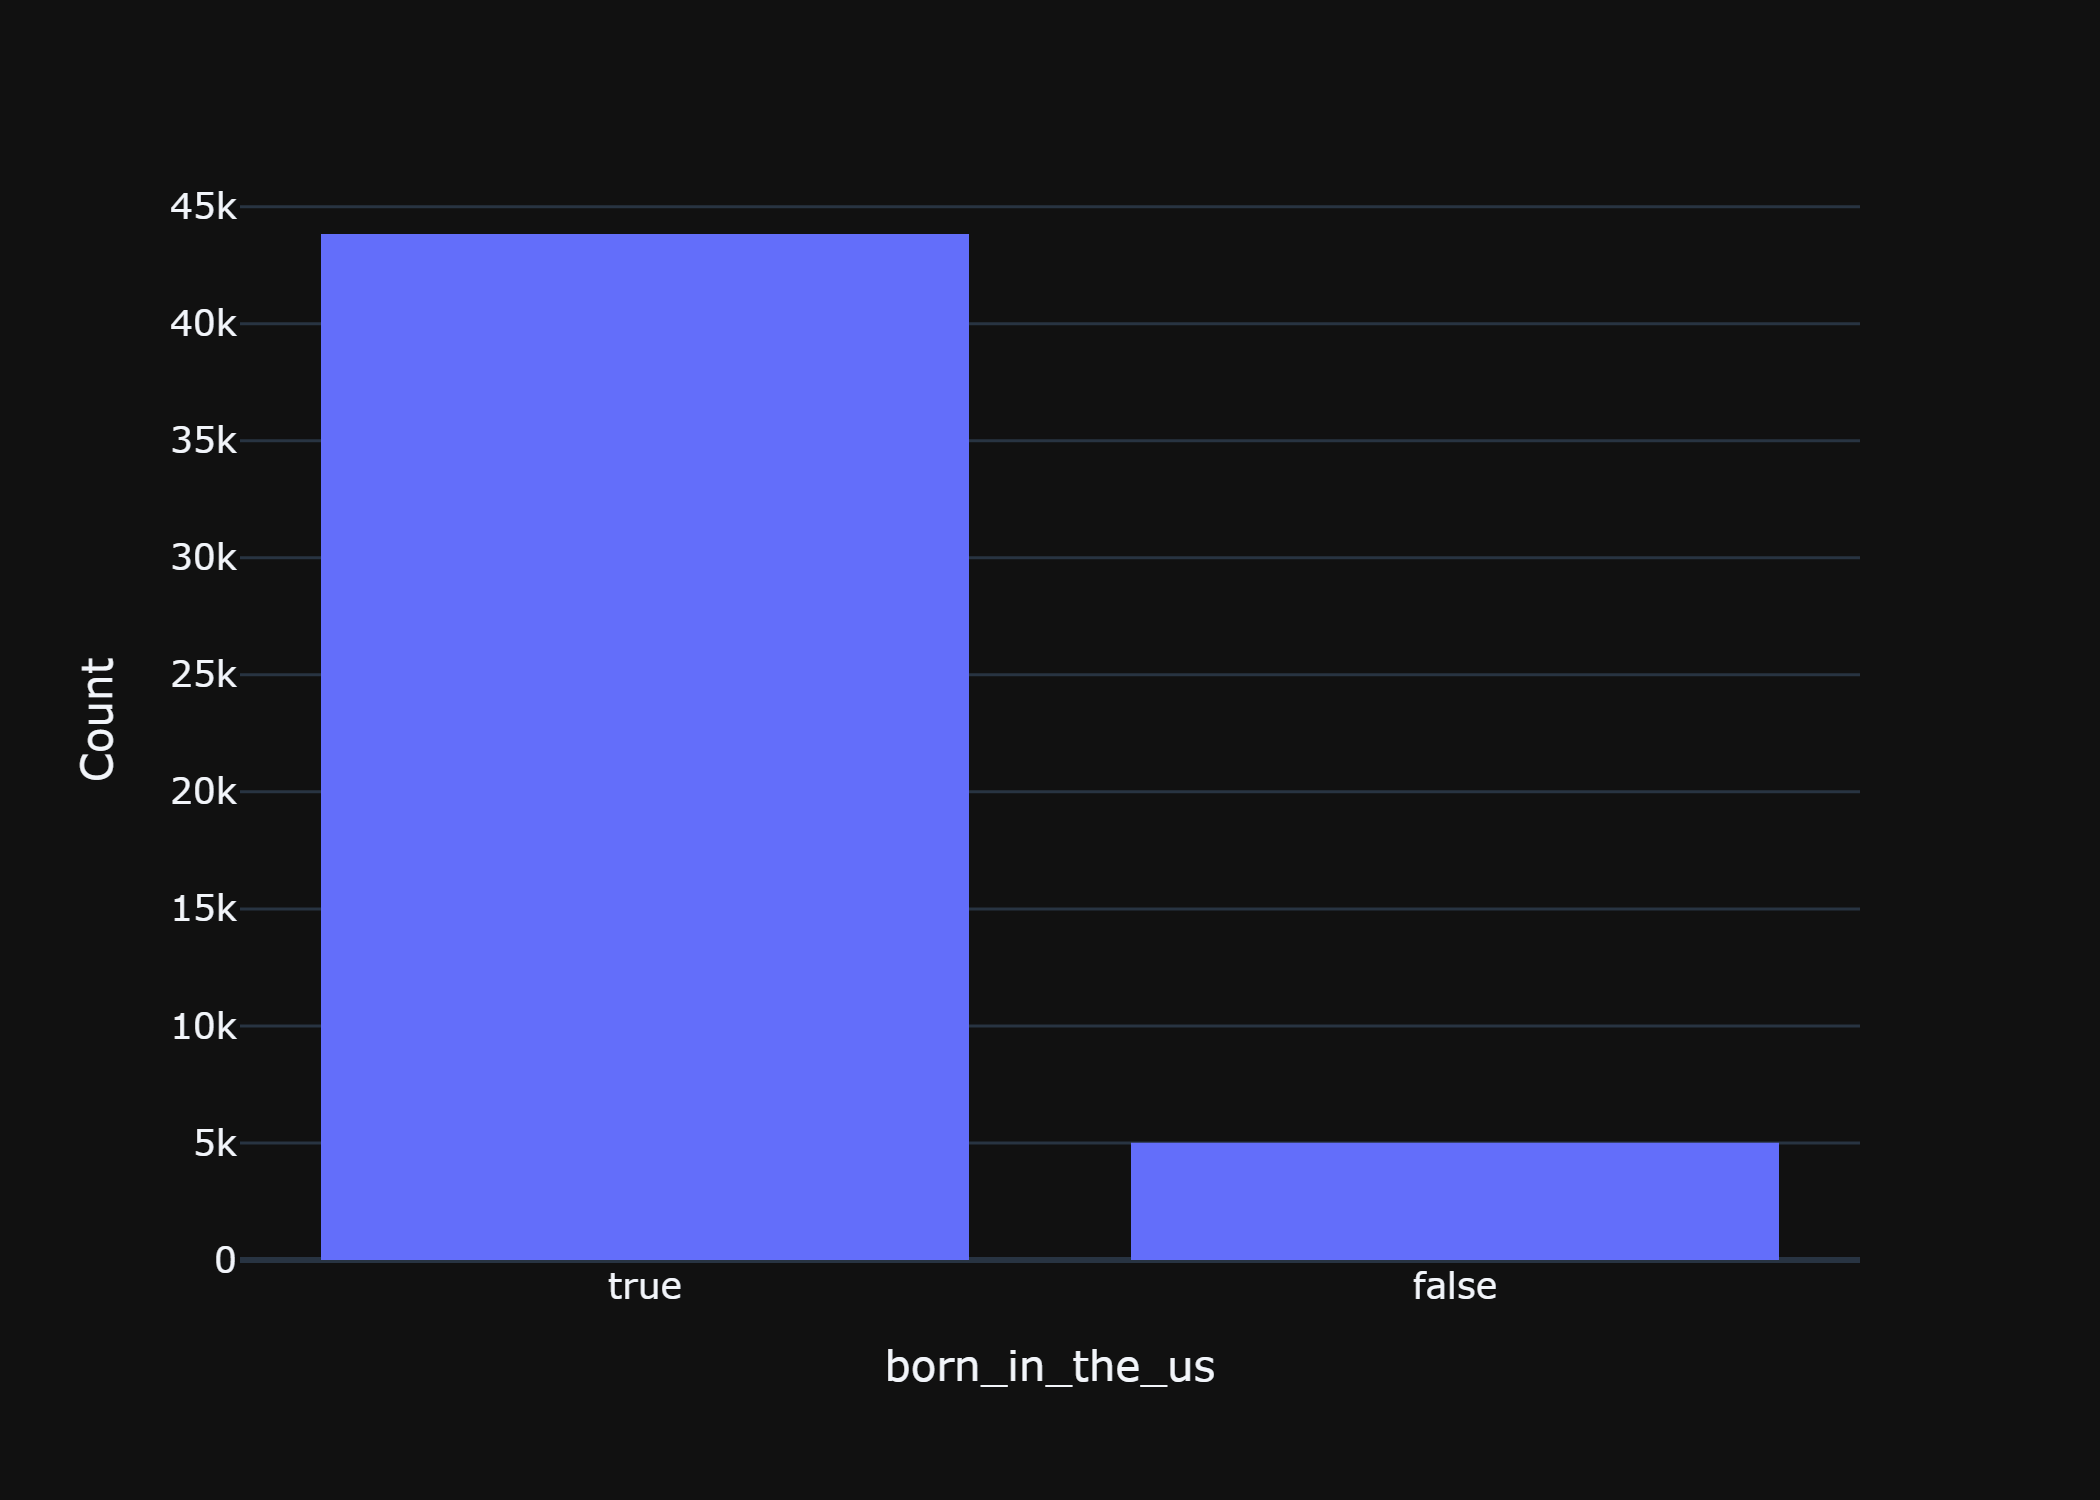
\includegraphics[width=0.8\textwidth]{Images/born_us.png}
    \caption{Distribution of people who are born in us or not}
    \label{fig:native_country}
\end{figure}


\textbf{Observation:}
The \texttt{native-country} feature exhibits extreme class imbalance (see Figure \ref{fig:native_country}). The United States represents approximately \textbf{90\%} of the observations, while the second most frequent country (Mexico) accounts for only \textbf{1.95\%}. The remaining 40 distinct countries constitute a "long tail" of sparse data.

\textbf{Feature Engineering Strategy:}
Applying standard One-Hot Encoding would result in over 40 new columns, most of which would be sparse and lack statistical significance due to low sample sizes. This would unnecessarily increase the model's complexity.

\textbf{Decision:} We opt for a **binary transformation** to capture the dominant signal:
\begin{itemize}
    \item We create a single boolean feature, \texttt{born\_in\_usa}.
    \item \textbf{Mapping:} Individuals born in 'United-States' are mapped to \texttt{1} (True). All other countries, including \texttt{NaN} values, are grouped into the minority class \texttt{0} (False).
\end{itemize}
This strategy preserves the most predictive information (domestic vs. foreign labor force) while drastically reducing dimensionality.

\section{Analysis of Hours per week}

\begin{figure}[H]
    \centering
    \subfigure[Distribution of hours per week]{
        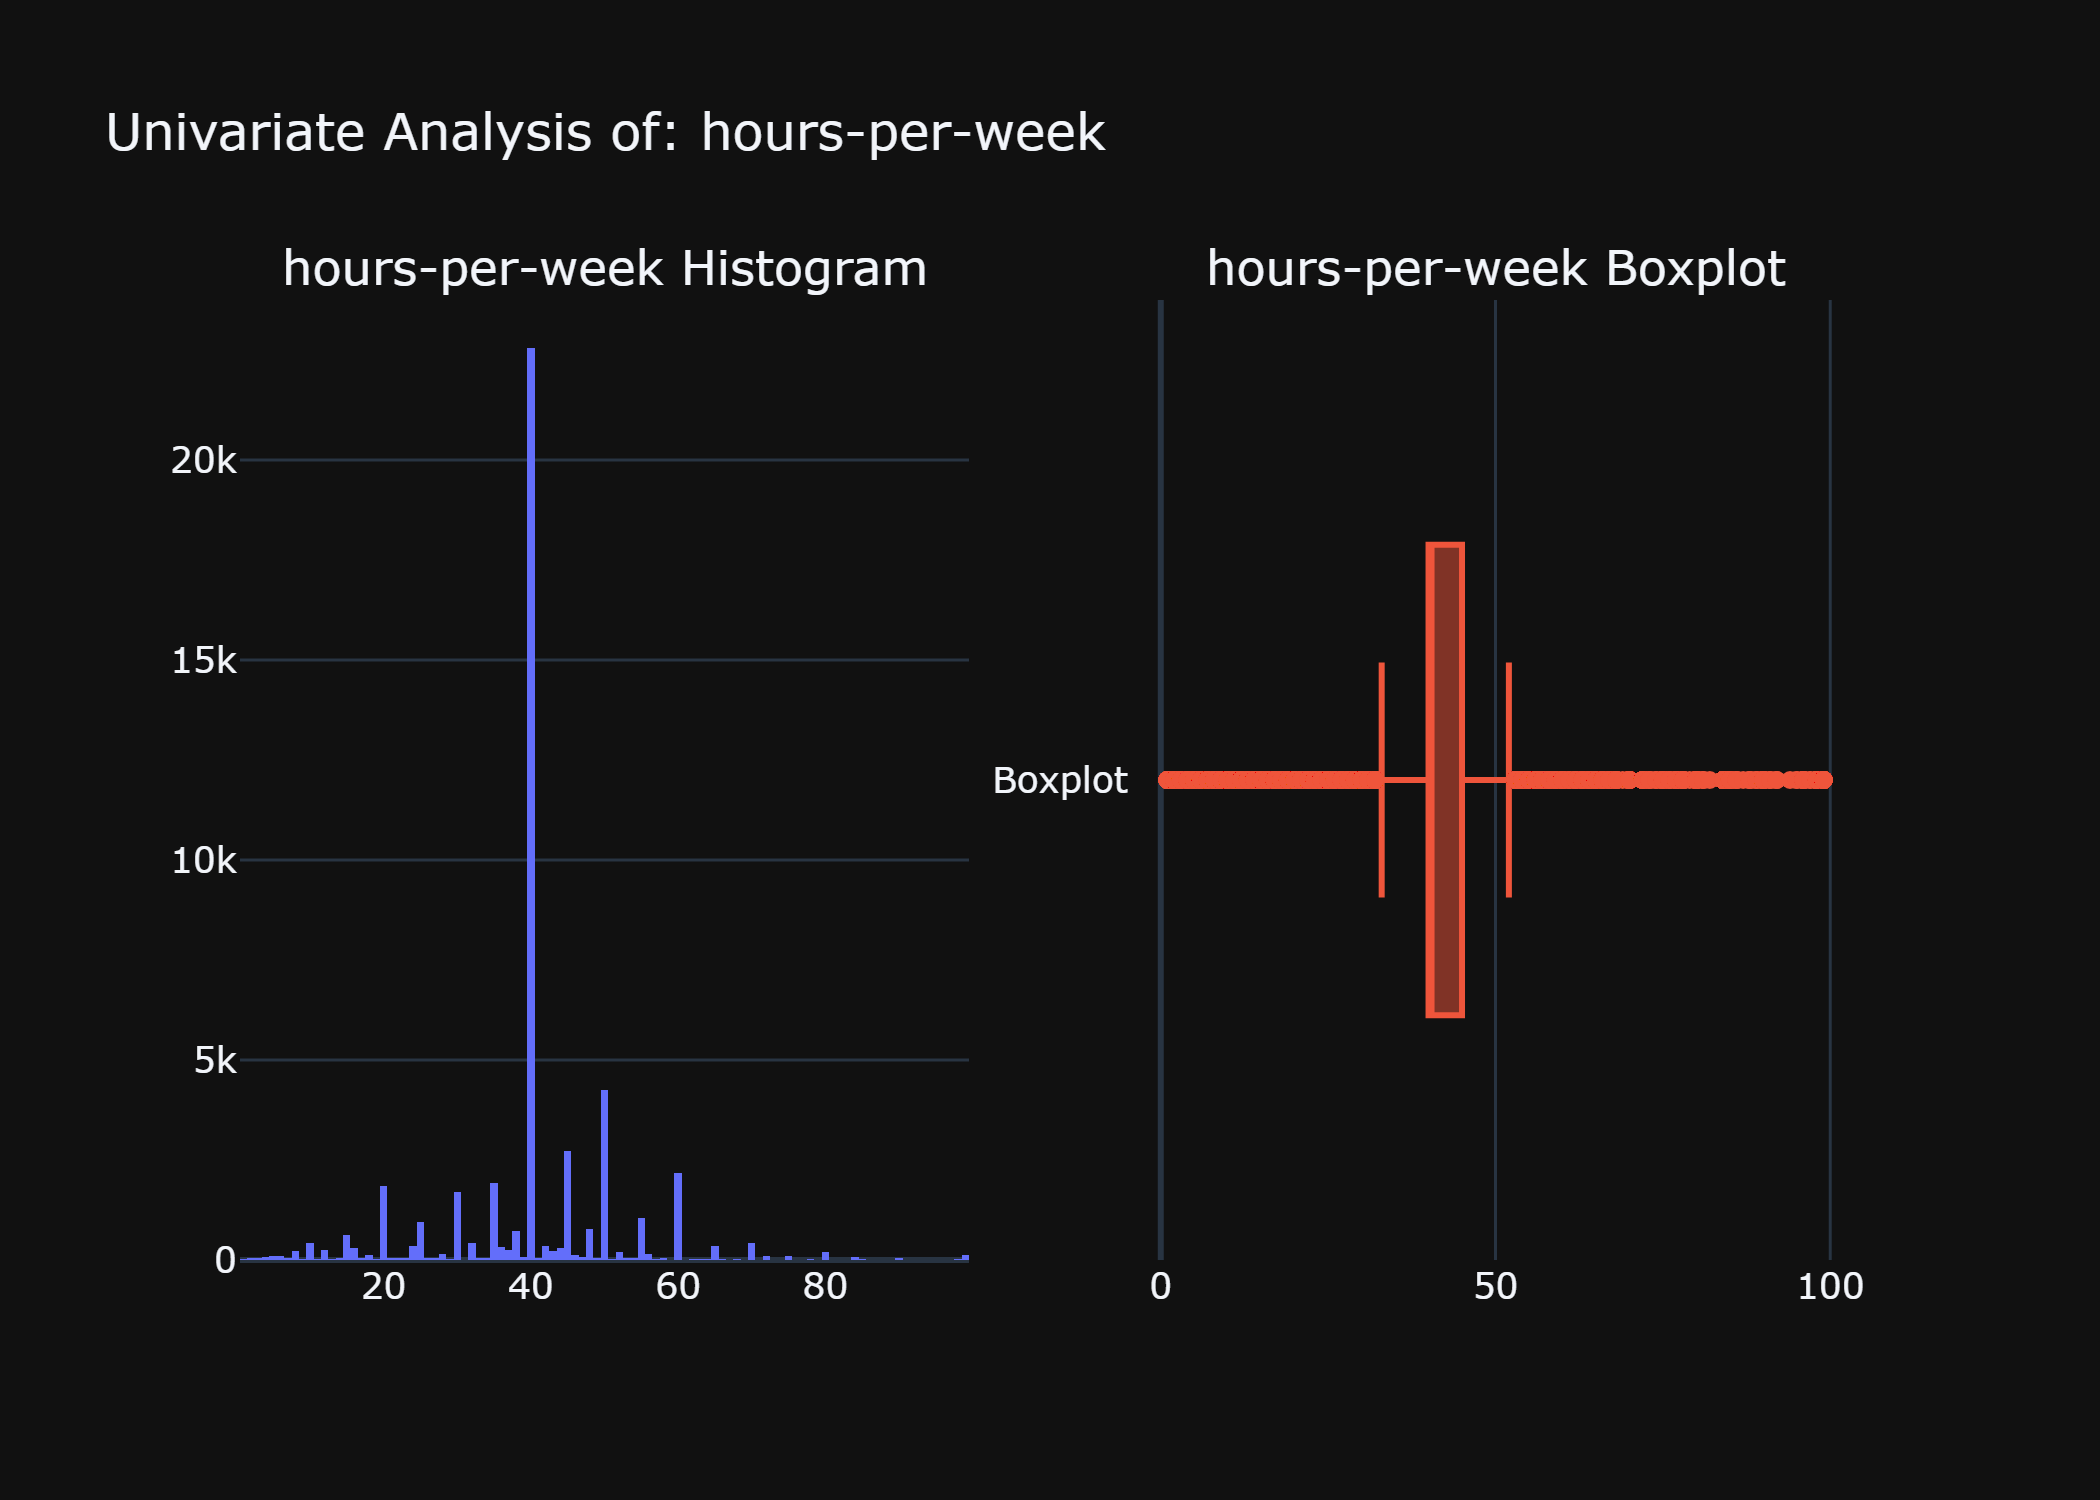
\includegraphics[width=0.45\textwidth]{Images/hours_per_week_hist.png}
        \label{fig:hours_analysis}
    }
    \hfill
    \subfigure[Relation between hours per week and income]{
        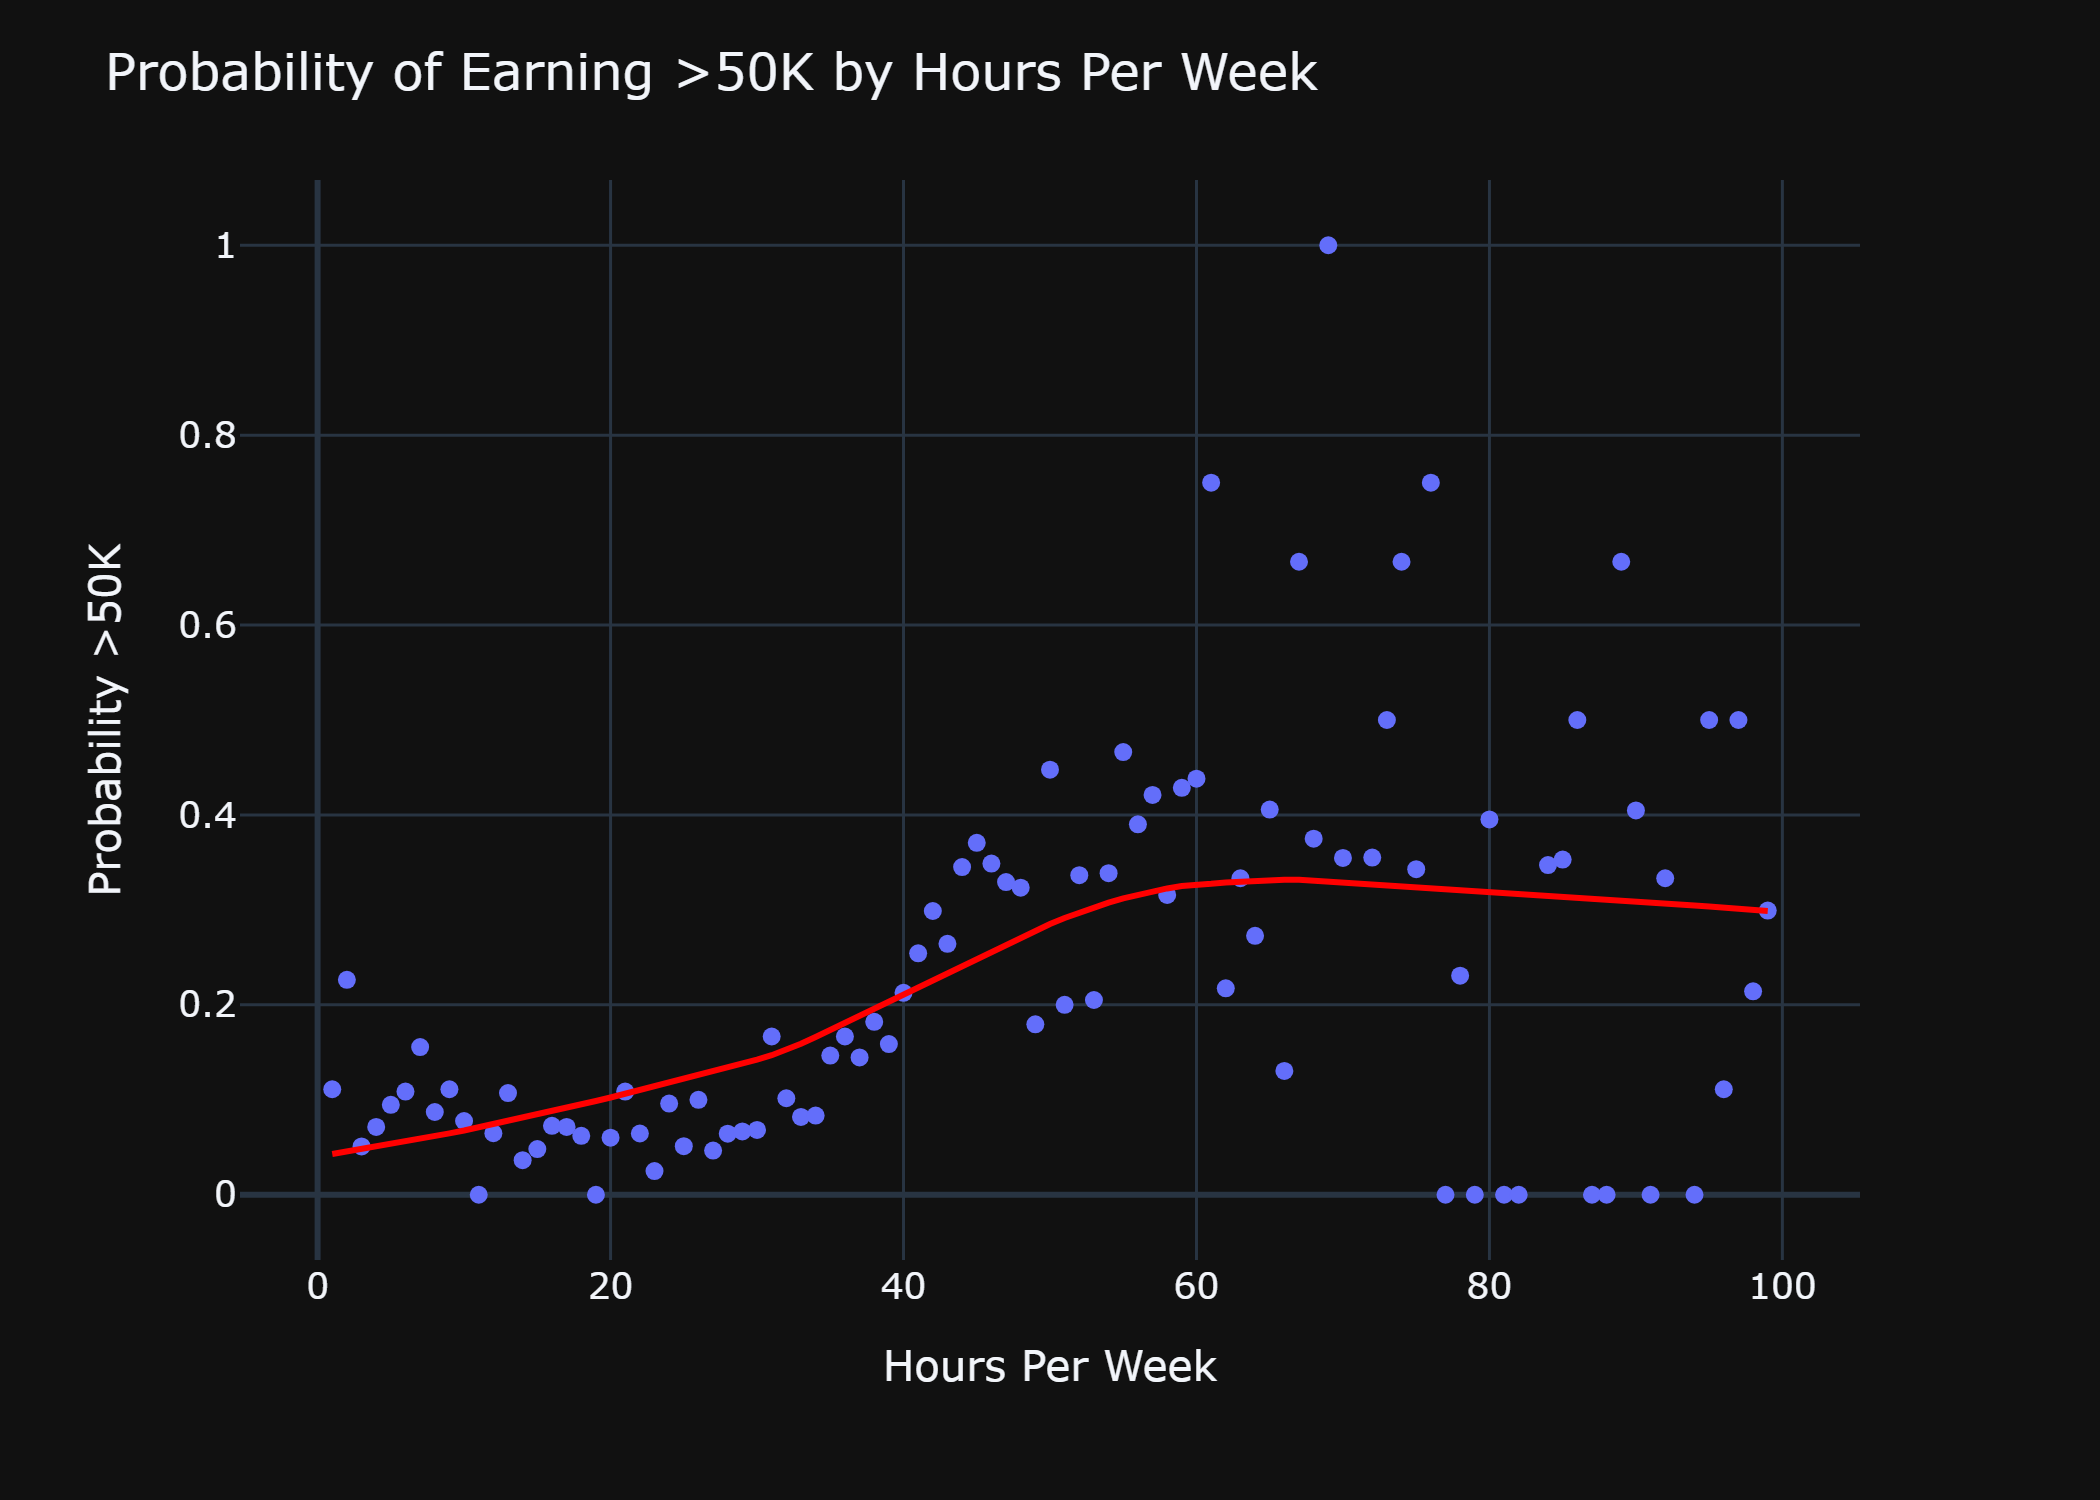
\includegraphics[width=0.45\textwidth]{Images/hours.png}
        \label{fig:hours}
    }

    \caption{Univariate analysis of the Hours per week feature and relation with income}
    \label{fig:hours_plots}
\end{figure}

\textbf{Observations:}
The distribution of \texttt{hours-per-week} (Figure \ref{fig:hours_analysis}) is distinctively leptokurtic, revealing two major structural insights:
\begin{enumerate}
    \item \textbf{The 40-Hour Norm:} An overwhelming majority of the population works exactly 40 hours per week, creating a massive central spike in the histogram.
    \item \textbf{High-Income Outliers:} The probability plot (Figure \ref{fig:hours}) shows that the likelihood of earning $>50K$ is low for part-time work, rises sharply at the 40-hour mark, and continues to increase for those working overtime (50--60 hours), before stabilizing.
\end{enumerate}

\textbf{Feature Engineering Strategy:}
Using the raw numerical value would force a linear relationship where "more hours = more money" at a constant rate, which fails to capture the specific "bonus" associated with hitting the full-time threshold.
\textbf{Decision:} We will apply **domain-specific discretization** to capture these three distinct economic behaviors:
\begin{itemize}
    \item \texttt{Part-Time} ($<40h$): Often correlated with lower hourly wages.
    \item \texttt{Standard} ($=40h$): The baseline for the majority of the workforce.
    \item \texttt{Overtime} ($>40h$): Strongly correlated with higher income and salaried positions.
\end{itemize}

\section{Analysis of Capital Loss and Gain}

\begin{figure}[H]
    \centering
    \subfigure[Distribution of Capital Gain]{
        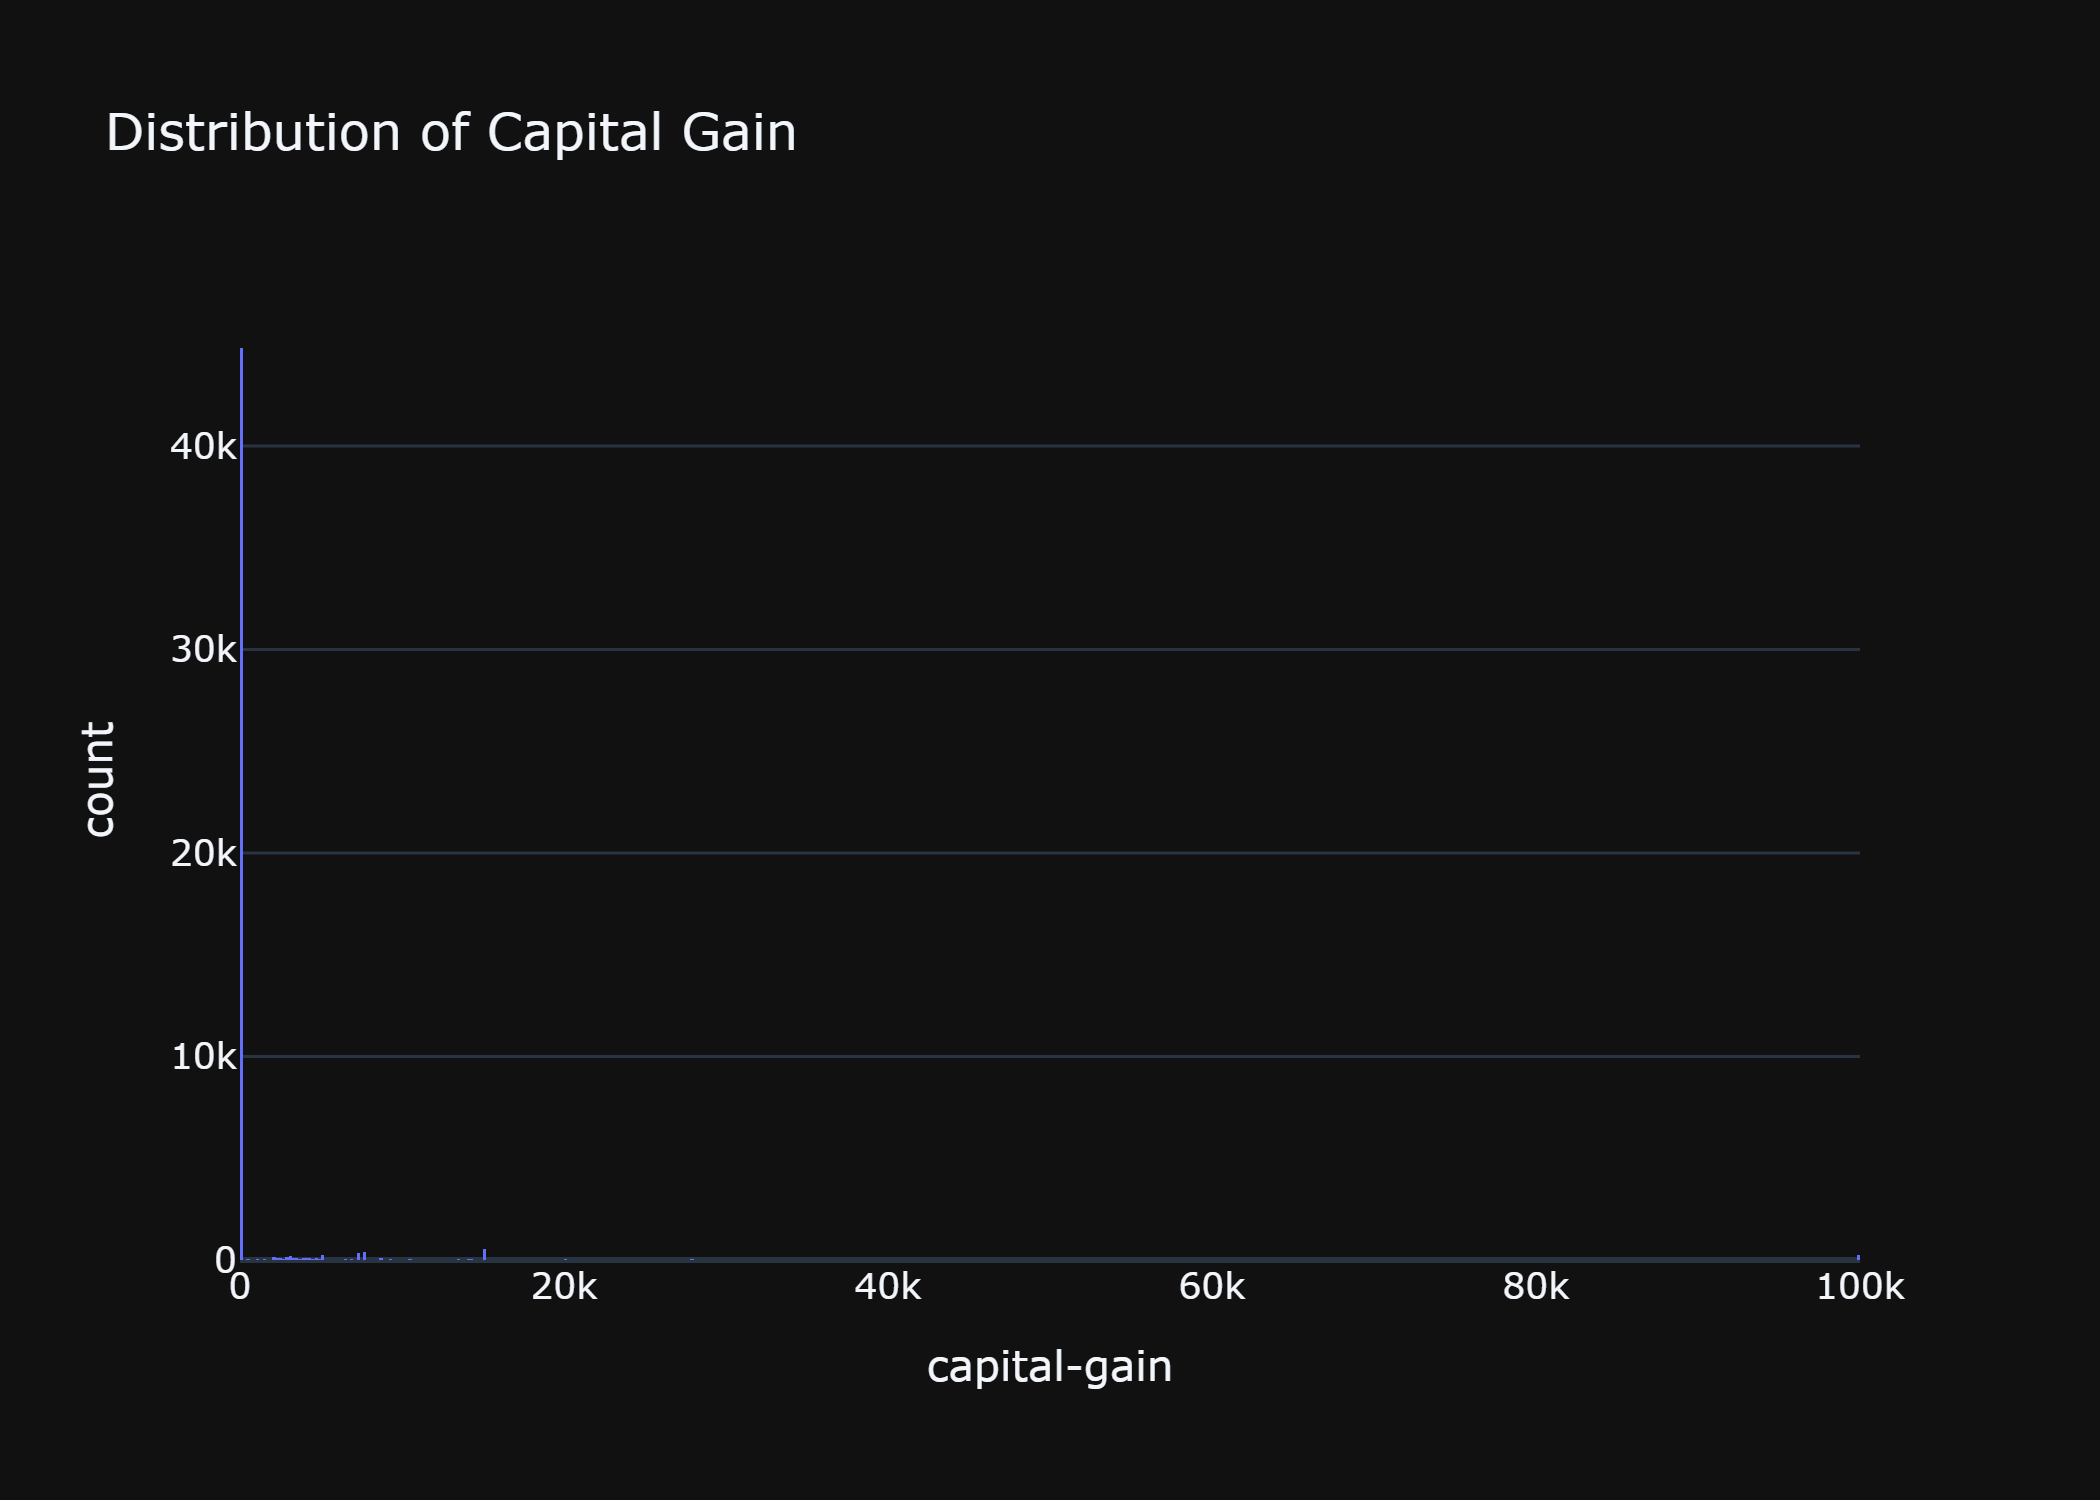
\includegraphics[width=0.45\textwidth]{Images/gain_distribution.png}
        \label{fig:gain_distribution}
    }
    \hfill
    \subfigure[Distribution of Capital Loss]{
        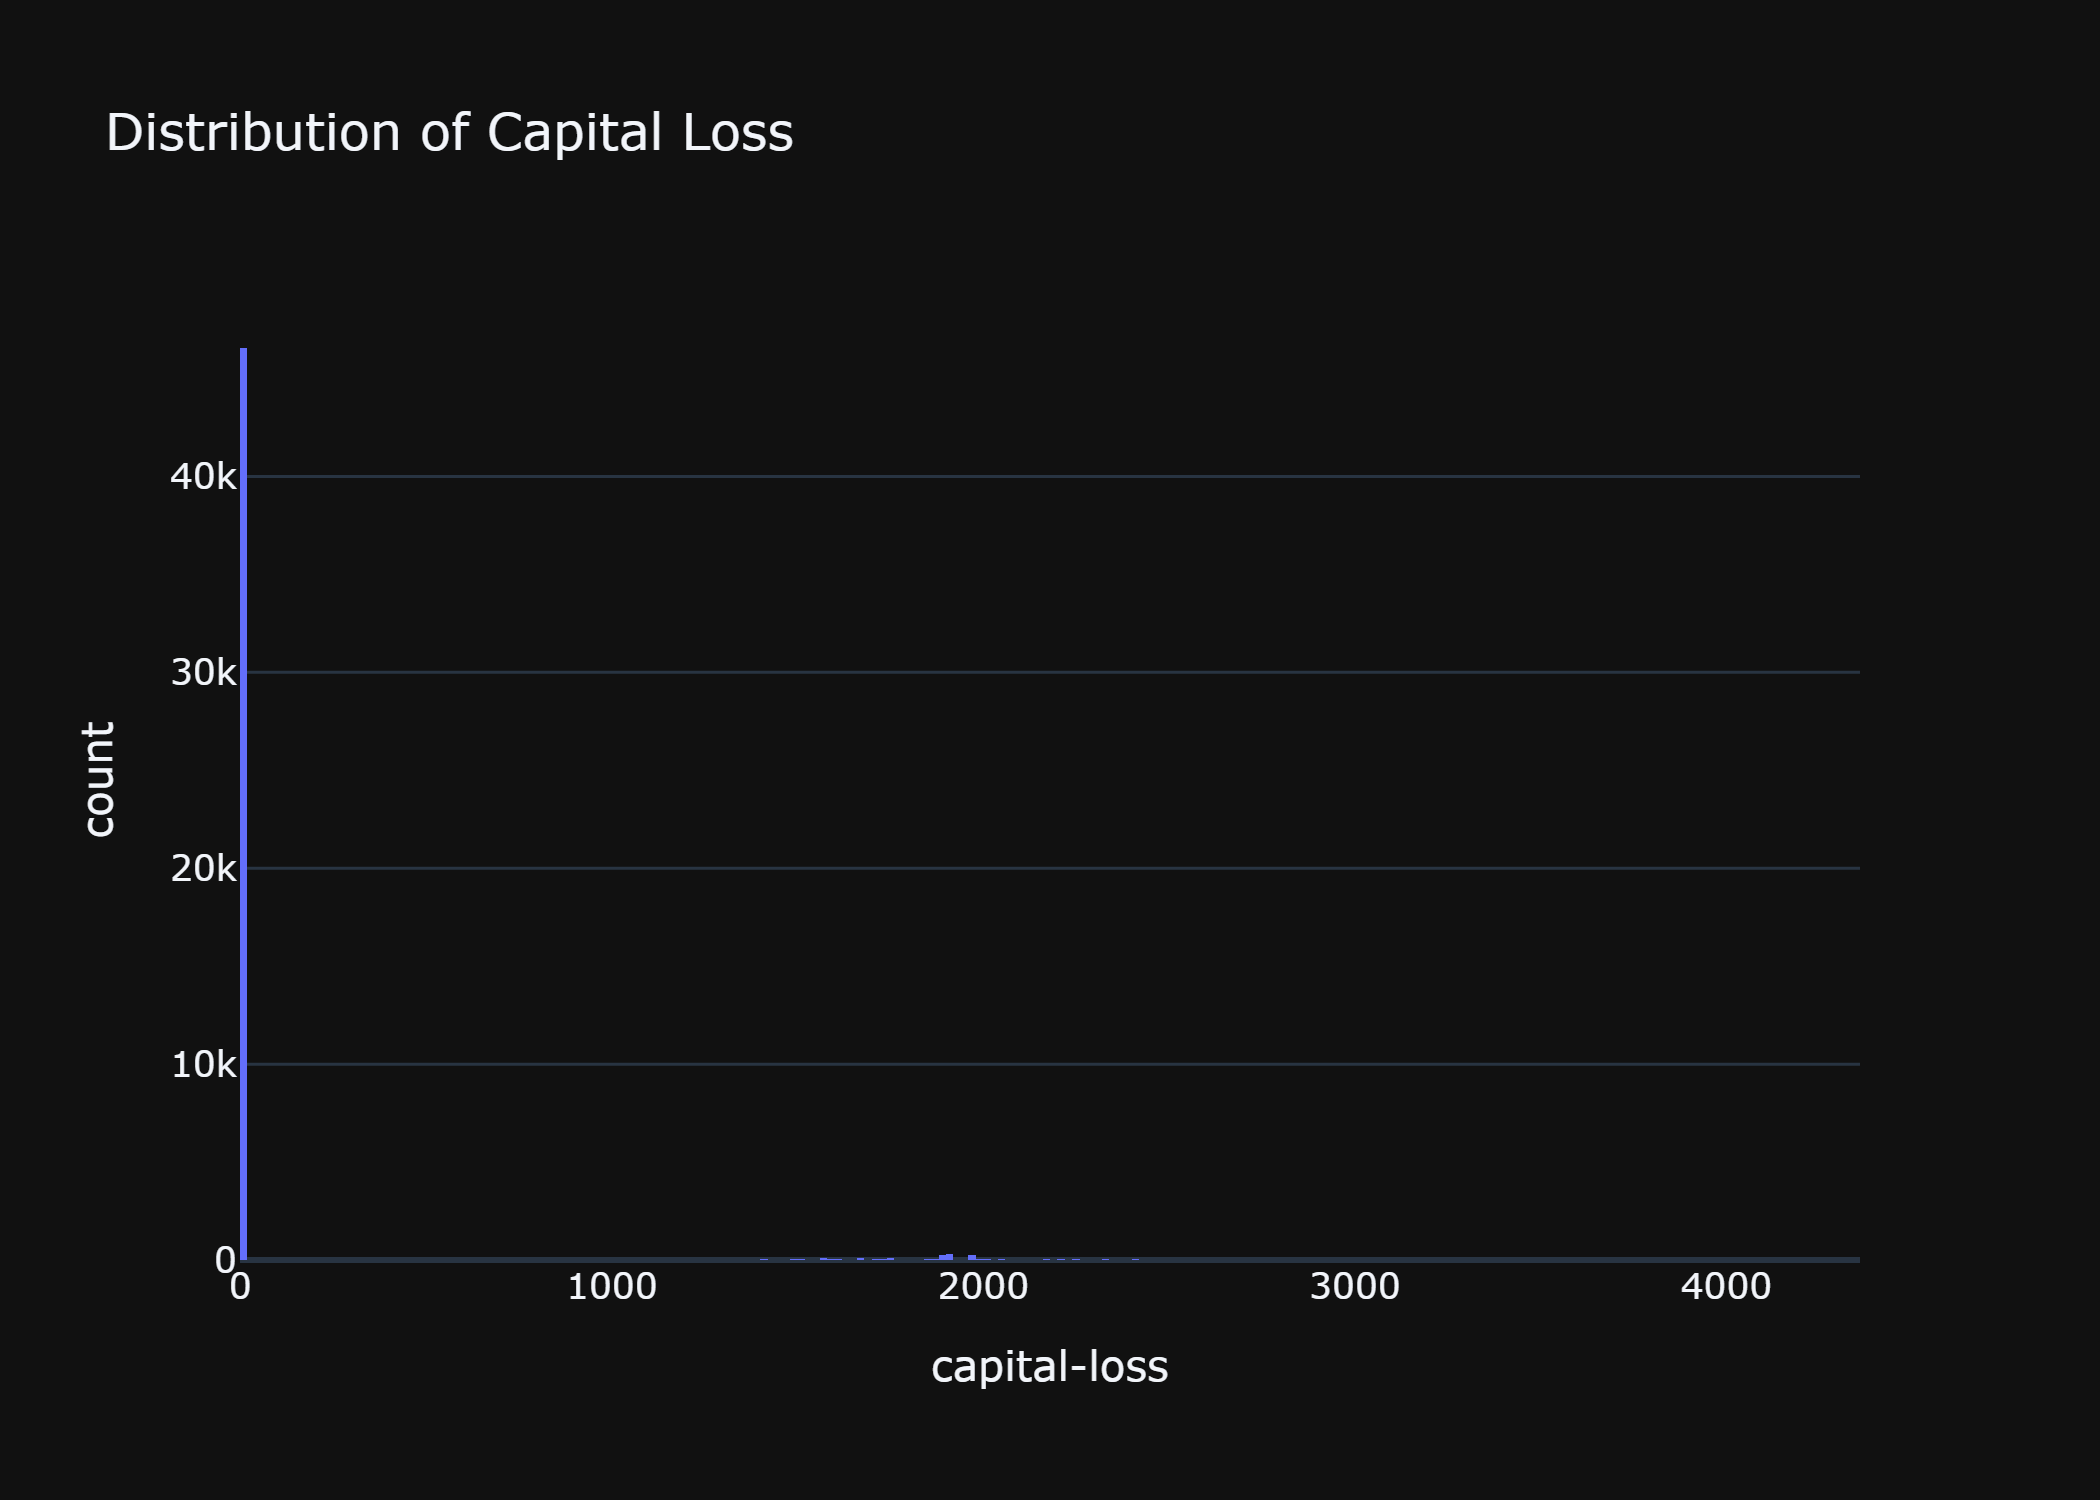
\includegraphics[width=0.45\textwidth]{Images/loss_distribution.png}
        \label{fig:loss_distribution}
    }

    \vfill
    \subfigure[Distrubution of Capital Change]{
        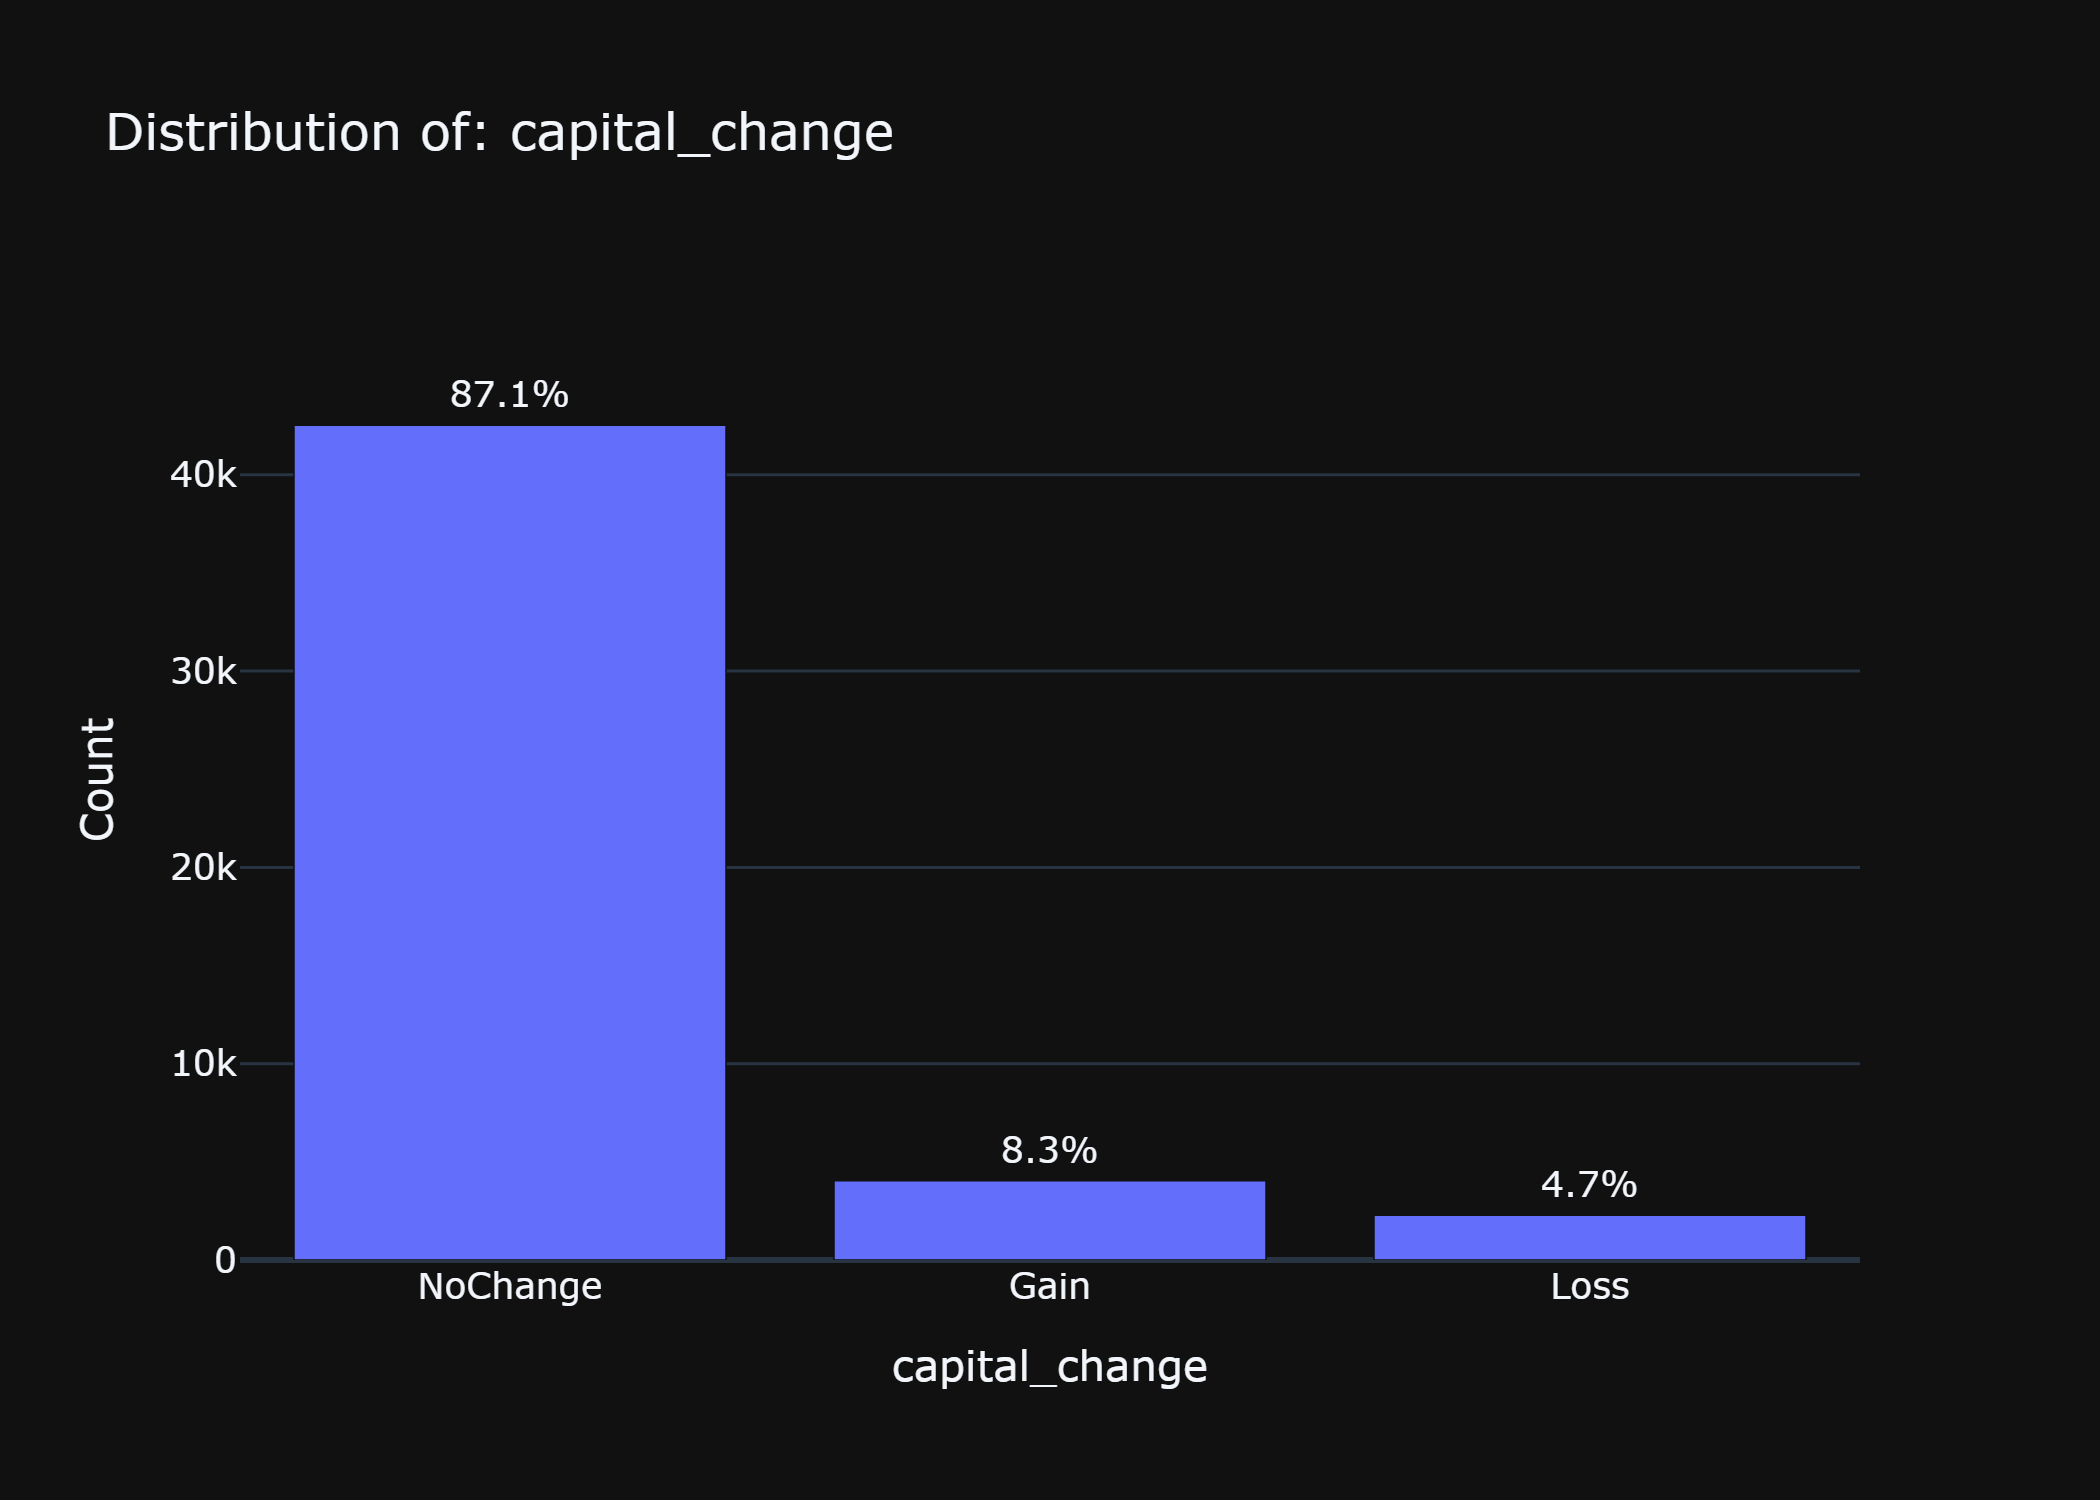
\includegraphics[width=0.45\textwidth]{Images/distribution_change.png}
        \label{fig:distribution_change}
    }
    \hfill
    \subfigure[Proportion of Income in Capital Change]{
        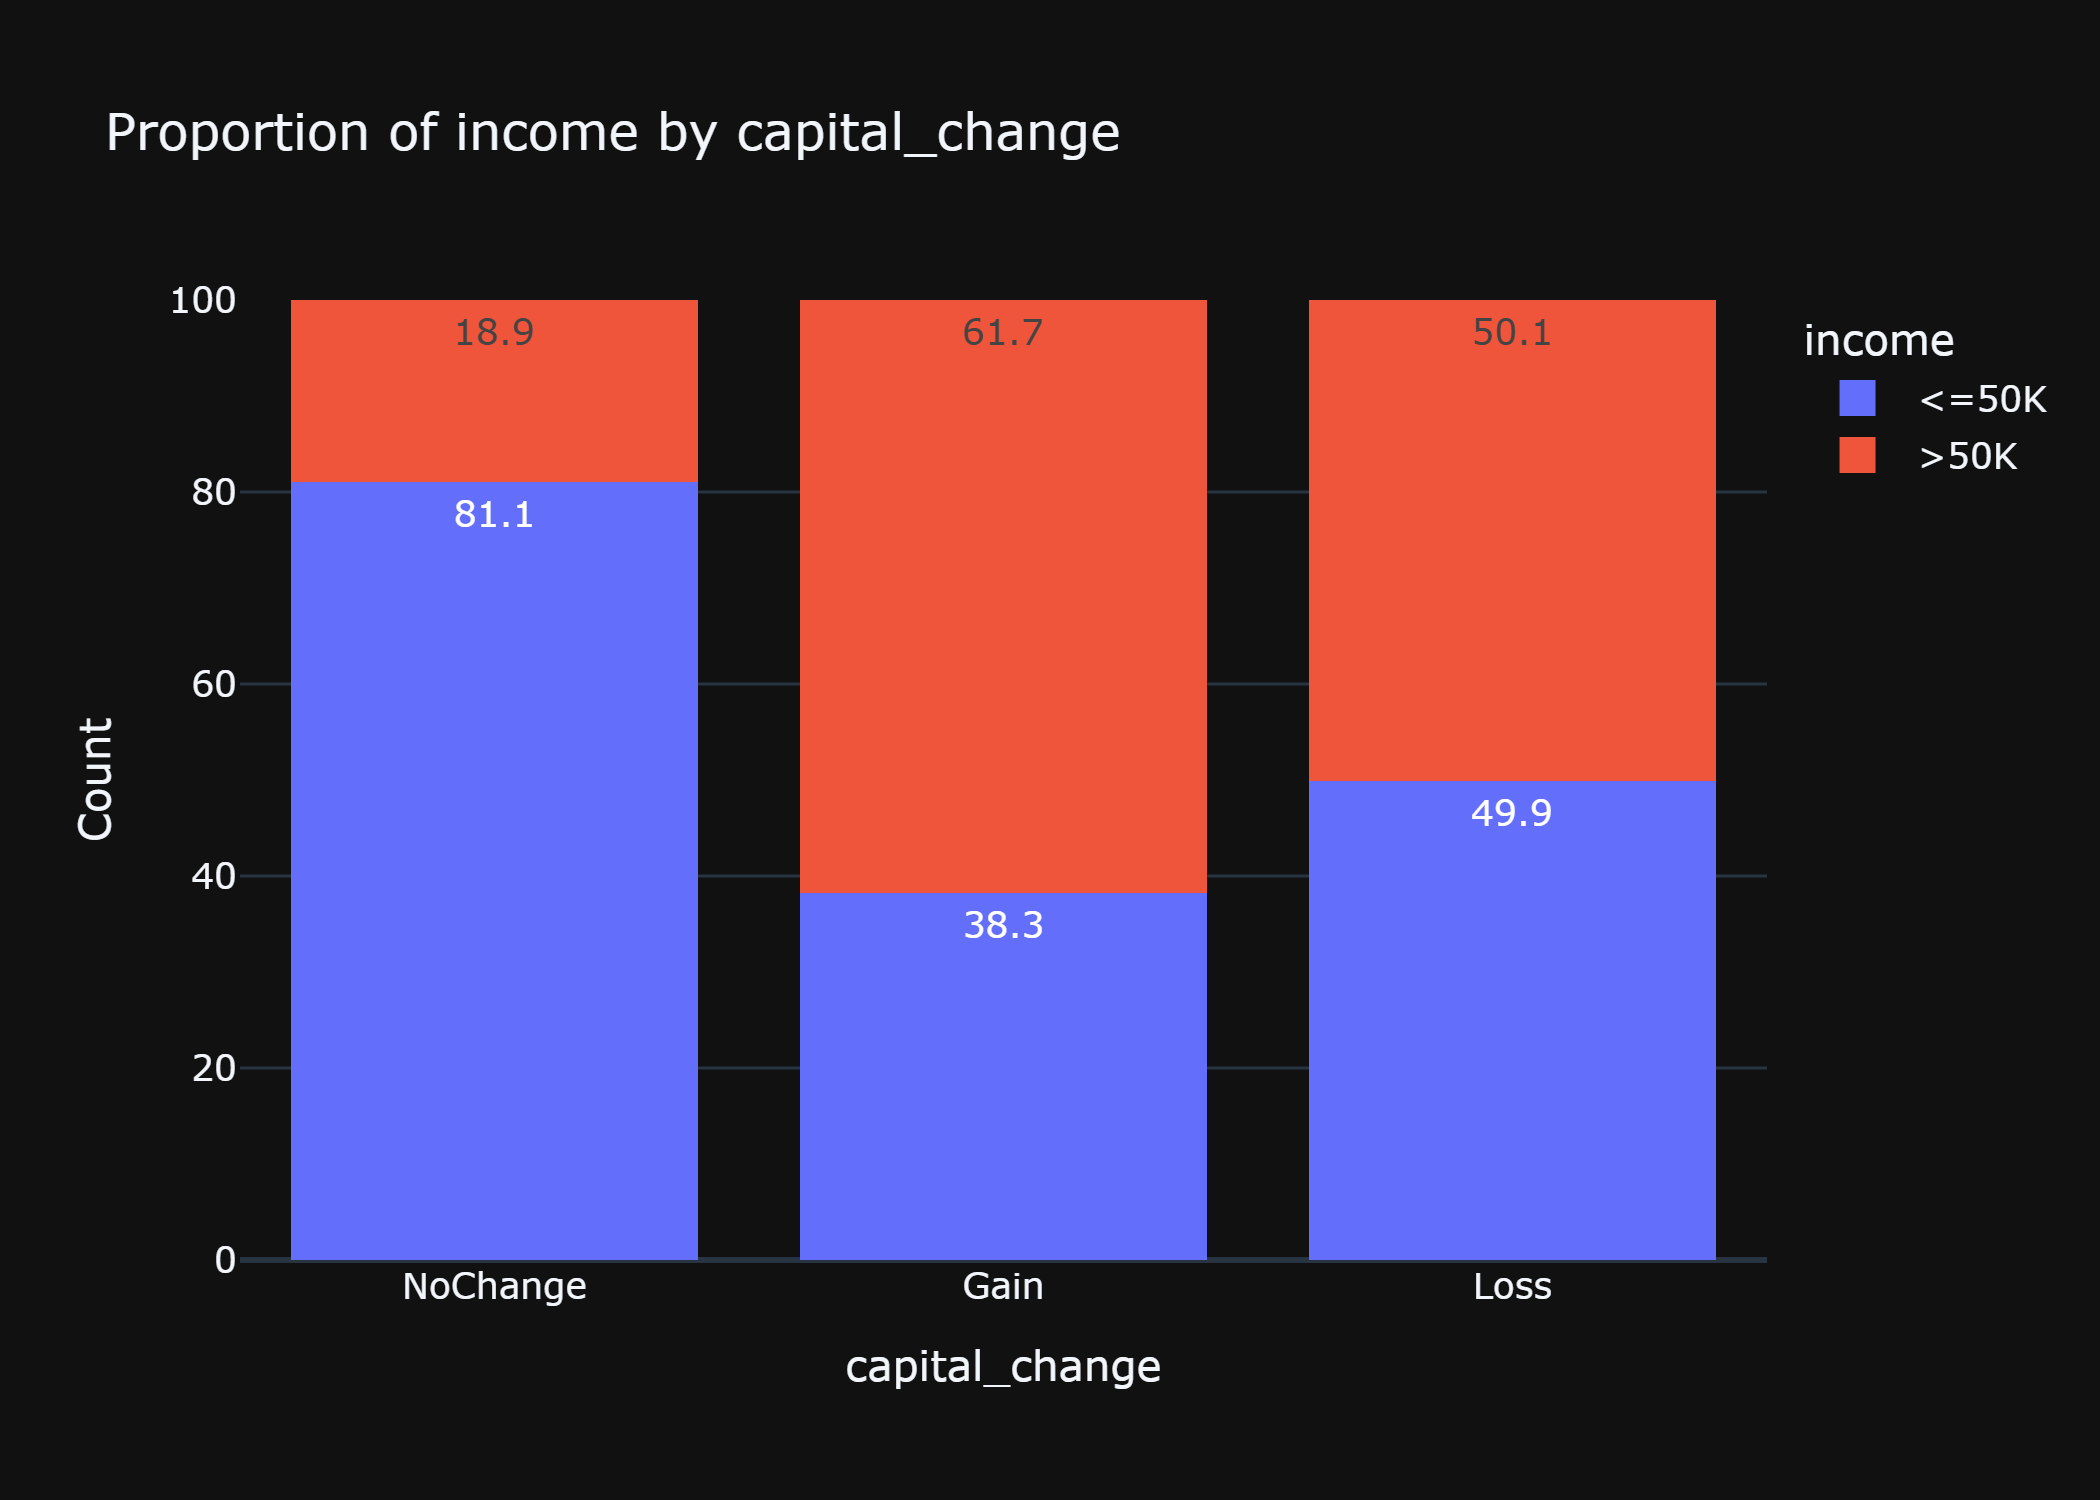
\includegraphics[width=0.45\textwidth]{Images/proportion_change.png}
        \label{fig:proportion_change}
    }


    \caption{Analysis of the Capital Gain and Loss}
    \label{fig:capital_change}
\end{figure}



\textbf{Observations:}
The features \texttt{capital-gain} and \texttt{capital-loss} present a specific challenge: they are extremely \textbf{sparse and zero-inflated}. The vast majority of individuals have no capital events recorded.

\textbf{Key Insight:}
Bivariate analysis reveals a counter-intuitive but logical pattern:
\begin{enumerate}
    \item \textbf{Gains:} Naturally strongly correlated with high income ($61.7\%$ earn $>50K$).
    \item \textbf{Losses:} Surprisingly, having a capital \textit{loss} is also a strong predictor of high income ($50.1\%$ earn $>50K$). This acts as a proxy for wealth: one must possess significant disposable capital to invest and subsequently lose it.
\end{enumerate}

\textbf{Feature Engineering Strategy:}
While a logarithmic transformation is typically used for skewed distributions, it would not solve the issue of extreme sparsity (thousands of zeros).
\textbf{Decision:} We move from a numerical to a \textbf{categorical approach}. We merge both columns into a single feature, \texttt{capital\_change}, with three distinct levels:
\begin{itemize}
    \item \texttt{NoChange}: The baseline majority.
    \item \texttt{Gain}: Indicates successful capital accumulation.
    \item \texttt{Loss}: Indicates active market participation.
\end{itemize}
This transformation simplifies the signal for the model, focusing on the \textit{existence} of capital assets rather than the magnitude.


\section{Heatmap \& Pairplot}

To conclude our Exploratory Data Analysis, we examine the relationships between features to detect redundancy (multicollinearity) and assess the
geometric complexity of the classification problem.

\subsection{Correlation Heatmap: Verifying Feature Independence}

\begin{figure}[H]
    \centering
    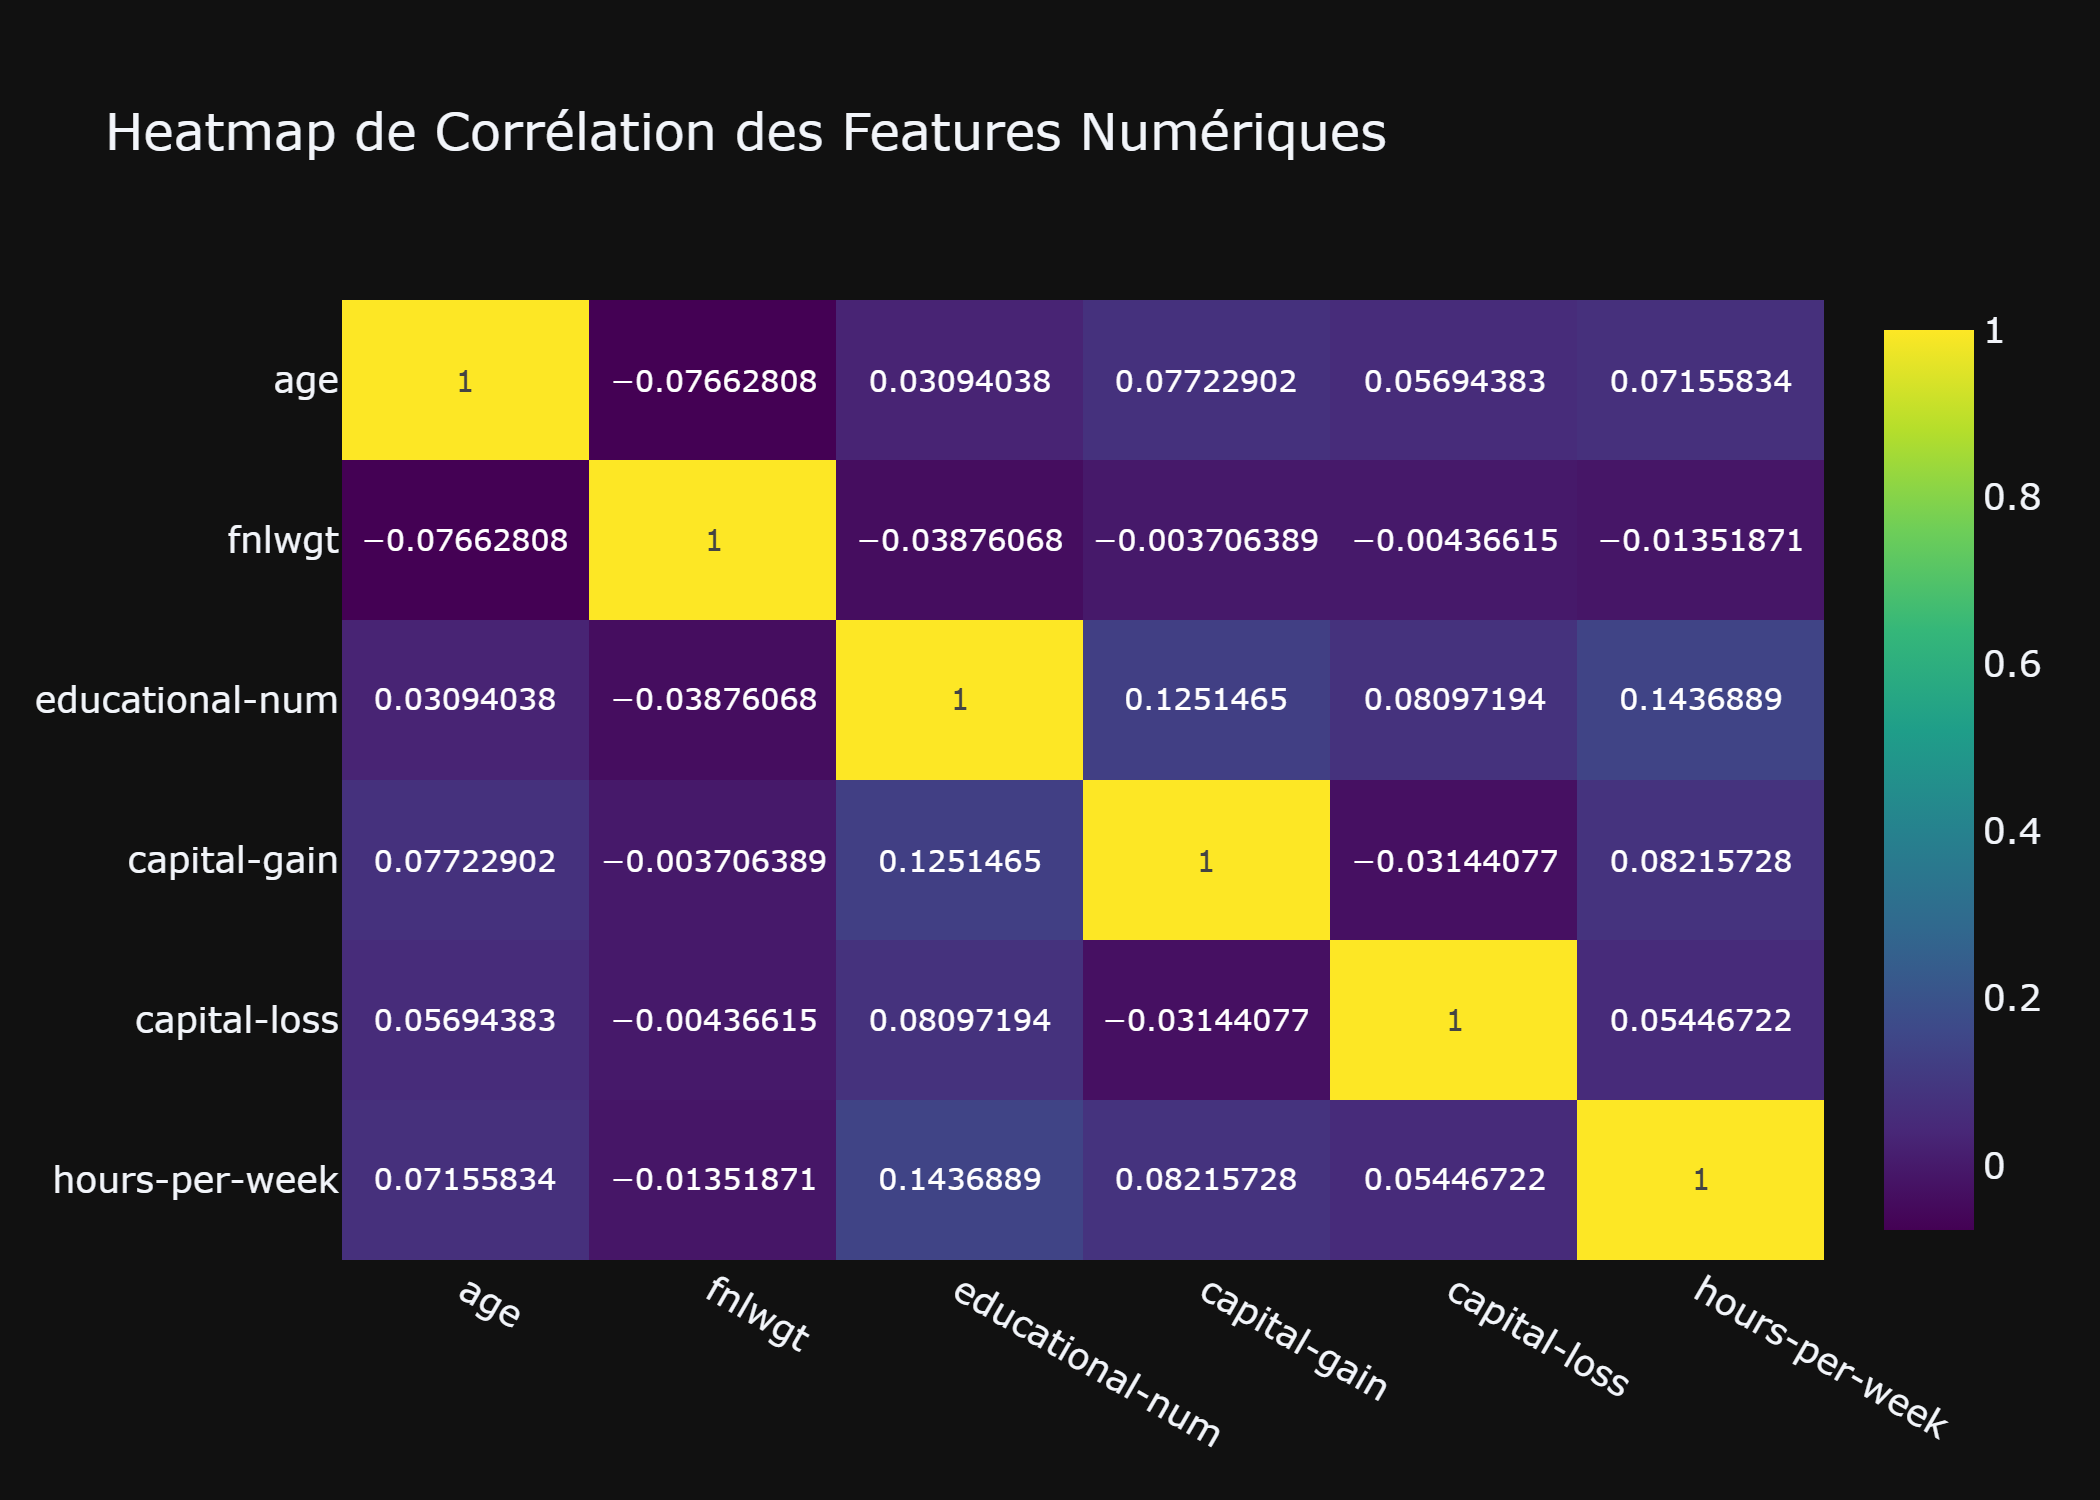
\includegraphics[width=0.8\textwidth]{Images/heatmap.png}
    \caption{Distribution of people who are born in us or not}
    \label{fig:heatmap}
\end{figure}

\textbf{Observation:}
The correlation matrix (Figure \ref{fig:heatmap}) reveals a remarkable absence of strong linear relationships between our numerical independent
variables.
\begin{itemize}
    \item \textbf{No Multicollinearity:} All correlation coefficients are extremely low, with the highest value being merely $\rho = 0.14$ (between \texttt{educational-num} and \texttt{hours-per-week}). This is well below the threshold ($>0.7$ or $0.8$) typically associated with multicollinearity issues.
    \item \textbf{Confirmation of Noise:} The \texttt{fnlwgt} feature displays near-zero correlation with all other variables (coefficients ranging from $-0.07$ to $-0.003$), reinforcing our previous univariate conclusion that it contains no predictive structure relative to other demographic factors.
\end{itemize}

\textbf{Conclusion:}

The lack of correlation implies that our numerical features are essentially orthogonal, each variable provides unique, independent information to the model. We do not need to drop any features due to redundancy.

\subsection{Pairplot Analysis: Assessing Separability}

\begin{figure}[H]
    \centering
    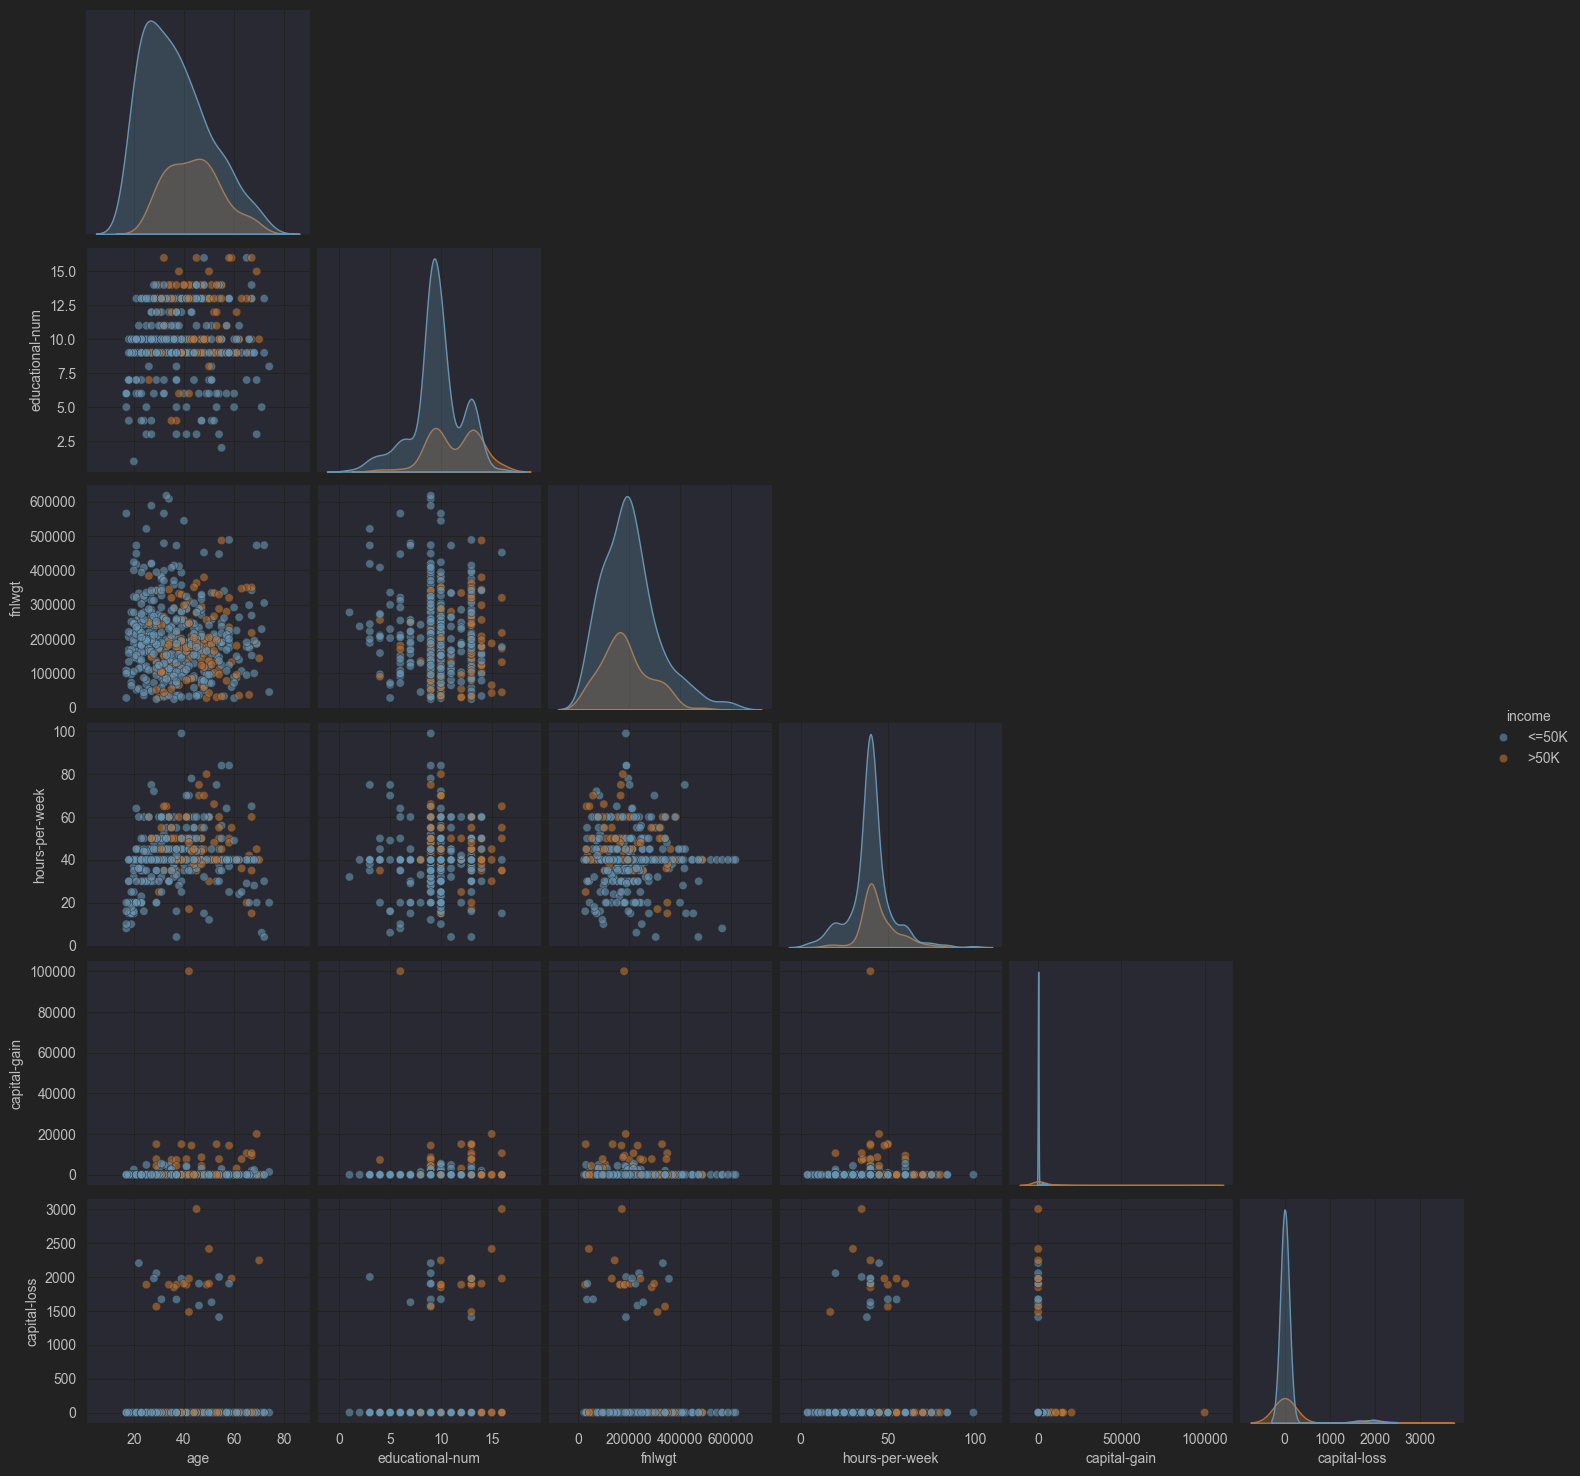
\includegraphics[width=0.8\textwidth]{Images/pairplot.png}
    \caption{Distribution of people who are born in us or not}
    \label{fig:pairplot}
\end{figure}

The Pairplot visualization (Figure \ref{fig:pairplot}) provides a global view of the interaction between features and the target class (\texttt{income}).

\textbf{Observations:}
\begin{enumerate}
    \item \textbf{Lack of Linear Separability:} There is no combination of two features where a simple straight line can clearly separate the two classes (blue vs. orange). The classes overlap significantly in the feature space.
    \item \textbf{Non-Linear Clusters:} Instead of linear trends, we observe dense clusters. For example, the interaction between \texttt{age} and \texttt{hours-per-week} forms a central "blob" where high earners are concentrated in the middle (middle-aged, full-time workers), surrounded by lower earners.
    \item \textbf{Confirmation of \texttt{fnlwgt} Irrelevance:} The plots involving \texttt{fnlwgt} show a completely random scattering of blue and orange points, confirming it acts as pure noise.
\end{enumerate}

\section{Conclusion of EDA}

Our exploratory analysis has established that while the raw data contains strong predictive signals (e.g., Age, Capital, Education),
these signals are often \textbf{non-linear, sparse, or categorical}.

Since the Pairplot demonstrates that the classes are not linearly separable in their raw form, simply feeding these variables into a linear
model (like Logistic Regression) would yield suboptimal results. To bridge this gap, we must proceed to \textbf{Feature Engineering}. Our goal will
be to restructure this information through binning, one-hot encoding, and noise reduction to create a dataset that maximizes the performance of
our machine learning models.








